\section{Eksperymenty numeryczne}
\label{section:eksperymenty}
  W celu weryfikacji proponowanych zmian skorzystałem ze standaryzowanych zadań optymalizacyjnych stosowanych w ramach konkursu
  \texttt{IEEE CEC'17} \cite{cec2017}. Ze względu na fakt, że jest to jeden z najbardziej popularnych zbiorów problemów testowych, uzyskałem
  możliwość względnie obiektywnego porównania moich pomysłów z klasyczną wersją algorytmu \texttt{CMA-ES} oraz jego modyfikacjami.\\
  \indent Problemy w ramach zestawu zadań podzielone są na funkcje: unimodalne, multimodalne oraz kompozytowe. Problemy kompozytowe są
  złożeniami problemów multimodalnych, które dodatkowo podlegają pewnym przekształceniom jak obrót czy translacja.
  Sposób w jaki funkcje testowe są skonstruowane ma na celu sprawdzić różne własności algorytmu, a w szczególności: odporność na zaszumienie funkcji celu,
  niewrażliwość na przekształcenia afiniczne lub wymiar zadania. \\
  \indent Porównanie testowanych metod sprowadza się do porównania, która z nich uzyskała mniejszą wartość funkcji celu przy ustalonym budżecie wywołań tej funkcji.
  Organizatorzy konkursu sugerują, aby wyniki testów przedstawiane były w postaci tabelarycznej, ale ze względu na większą czytelność zdecydowałem się przedstawiać je za pomocą krzywych ECDF (ang. \textit{Empirical Cumulative Distribution Function}). Krzywa ECDF konstruowana jest w taki sposób, że na osi odciętych odkładany jest odsetek posiadanego budżetu wywołań funkcji, a na osi rzędnych -- procent problemów rozwiązanych przy zadanym budżecie przez algorytm. Im większe jest pole pod krzywą danego algorytmu, tym lepszy wynik uzyskał on względem pozostałych metod.
  

\subsection{Parametry eksperymentów}
  W ramach eksperymentu porównałem proponowane przeze mnie metody z algorytmem \texttt{CMA-ES} w klasycznej postaci (t.zw. \texttt{CSA-CMA-ES}) oraz z algorytmem \texttt{MSR-CMA-ES}.
  Wszystkie wspólne parametry metod jak rozmiar populacji $\lambda$ są zgodne z zalecaniami przedstawionymi przez autora algorytmu w \cite{CMADEhansen}.
  Specyficzne parametry algorytmu \texttt{MSR-CMA-ES} ustalono zgodnie z sugerowanymi wartościami w \cite{Elhara13}. Algorytmy testowano dla zadań o wymiarowości $D = 10, 30$ przy budżecie wywołań funkcji celu równym $10^{4}D$.

\subsection{Wyniki na standaryzowanych problemach testowych}

Na Rys. \ref{cec-17} przedstawione są uzyskane wyniki. Standardowa wersja algorytmu \texttt{CMA-ES} przewyższa wszystkie inne
rozważane w artykule modyfikacje tej metody. Reguła \texttt{CPEF} charakteryzuje się najgorszą wydajnością. Ogólna wydajność \texttt{PPMF} jest porównywalna z \texttt{CPMF}, z niewielką przewagą \texttt{PPMF} nad \texttt{CPMF}. Obie metody dają lepsze wyniki niż \texttt{MSR-CMA-ES}.

\begin{figure}[h]
\begin{centering}
\includegraphics[width = 0.65\textwidth, angle = 270]{cec-17.eps}
\end{centering}
\caption{Krzywe ECDF uzyskane dla wszystkich problemów zdefiniowanych w konkursie \texttt{CEC'17}}
\label{cec-17}
\end{figure}





